\chapter{SMT theories \& Symbolic Execution}
\section{Intro}
Validity in first order logic (FOL) is undecidable, while validity in particular first order theories is (sometimes) decidable. These theories allow us to capture structures which are used by programs (arrays, ints etc.) and enable reasoning about them. \\
Formulas in each theory are constructed with a specific set of function, predicate and constant symbols. This is the \underline{signature} of the theory called $\Sigma$. Using $\Sigma$, logical connectives ($\wedge, \to$) and quantifiers first order formulas can be built. Each theory comes with a set of \underline{axioms} (FOL formulas) called $A$, which only contain elements form the signature. A formula F in the theory \underline{is valid} if all interpretations that satisfy the axioms in $A$ also satisfy the formula. Some theories are meant to be used with a \underline{particular interpretation} (e.g. in theory of integers formulas are interpreted over ints). A \underline{fragment} of a theory consists of a subset of the possible formulas expressible in the theory. A theory is \underline{decidable} if for every formula in the theory we can automatically check whether the formula is valid or not. Similarly for fragments of a theory.
\section{Decidability}
Decidability is mainly needed to achive 100\% \underline{automation}. If the theory is not decidable sometimes the theorem prover (e.g. Z3, Yices) which is used may succeed.
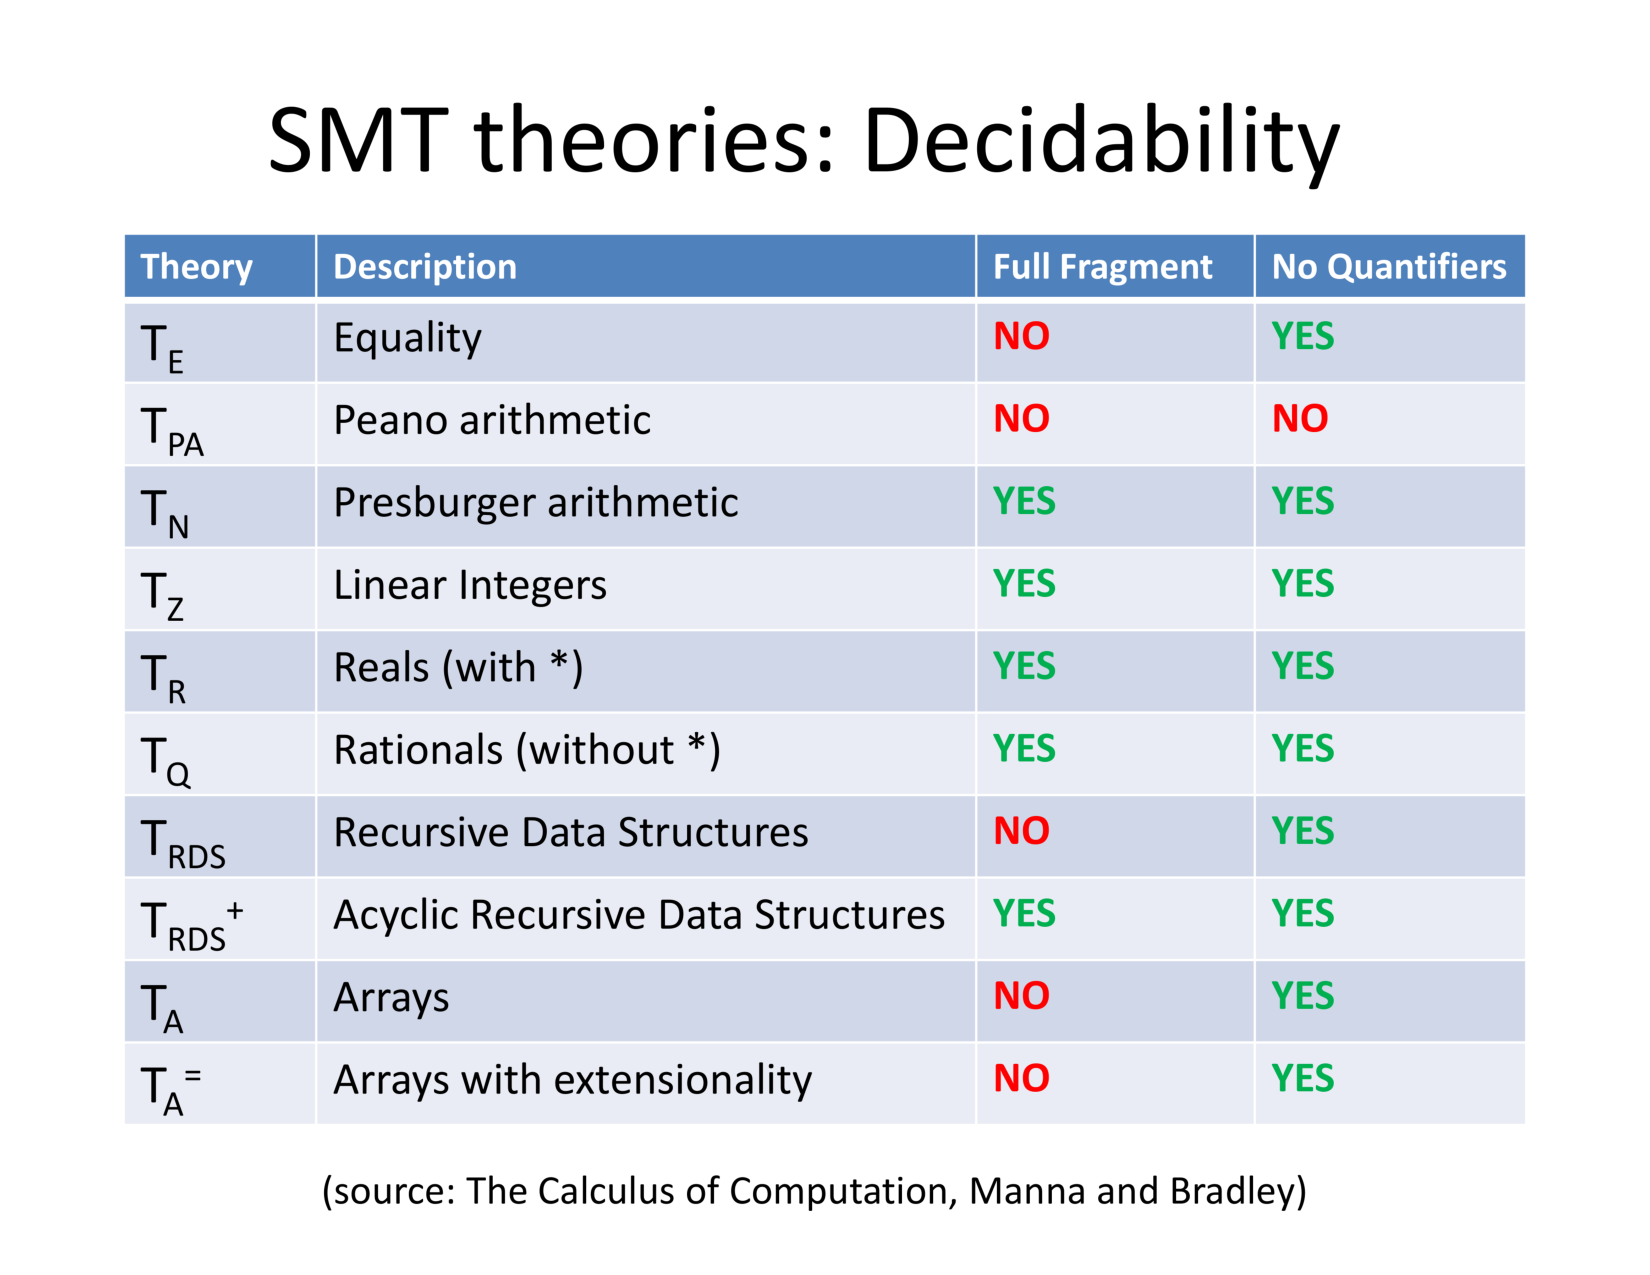
\includepdf[pages={-}]{pages/decidability.pdf}
\section{TODO}
pages <24 with all those theories.
\section{Symbolic Execution}
Widely used in practice. Symbolic Execution keeps two formulas at any point during program execution: \textbf{symbolic store} and a \textbf{path constraint}. The \underline{symbolic state} is the \underline{conjuction} of these two formulas.
\subsection{Existing Tools}
Stanford's KLEE, NASA's Java PathFinder, Microsoft Research's SAFE, UC Berkeley's CUTE, EPFL's S2E.
\subsection{Symbolic store}
$\sigma_s:Var \to Sym$ maps each variable to a value at any given time. Example: $\sigma_s: x \mapsto x0, y \mapsto y0$
\subsection{Semantics}
Arithmetic expression evlauation simply manipulates the symbolic values. Let $\sigma_s: x \mapsto x0, y \mapsto y0$ Then, $z=x+y$ will produce the symbolic store: $x \mapsto x0, y \mapsto y0, z\mapsto x0+y0$ 
\subsection{Path Constraint}
Records all branches taken so far. Typically a decidable logical fragment without quantifiers. Is \underline{true} at the start of the analysis. Evaluation of \underline{conditionals} affects the path constraint but not the symbolic store.
\subsection{Limitation: Loops}
Unbounded loops run forever in symbolic execution. Easiest soluton: provide some loop bound meanging \underline{under-approximate}(under-approximation: only feasible paths?\textbf{TODO}). Another solution is to provide \underline{loop invariants}. But this is rarely used for large programs because it's difficult to provide such invariants manually and it can lead to \underline{over-approximation}. \underline{Static analysis can infer loop variants.} 
\subsection{Constraint solving}
It's important that
\begin{enumerate}
\item  a SMT solver suppoerts as many decidable logical fragments as possible (some tools even use more than one SMT solver)
\item  a SMT solver can solve large formulas quickly
\item the symbolic execution engine tries to reduce the burden in calling the SMT solver by exploring domain specific insights.
\end{enumerate}
A key-optimization is obviously \underline{caching}. The symbolic execution engine can keep a map (cache) of formulas to a satisfying assignment for the formula. For new formulas it can the first access the cache before calling the SMT solver.
\subsection{Concolic Execution - When constraint solving fails}
SMT solvers do not handle \underline{non-linear constraints} well (e.g z = y*y, ... page 47).
Concolic Execution combines \underline{both} symbolic execution and concrete (normal) execution. The program runs as usual (with some input that needs to be given) and also maintains the symbolic information. For example when there's a \textit{read()} use two stores. one with actual values (e.g. 22,1, etc.) and one with the symbolic information. Run several times. If for example the then branch is reached and we need the else brnach. negate path constraint and run againe. See examples on page 49.